%!TEX root = egalitarianism.tex

\section{Defining egalitarianism}\label{sec:definition}

Having established the basics of consensus mechanisms, we now propose the first
definition of an economic measure of \emph{egalitarianism} in cryptocurrencies.
Before we present our definition, let us first state the desiderata of such a
definition. First of all, we want to allow concrete measurements to be
performed on cryptocurrencies and data to be extracted in a manner that is
quantitative and not vague. Thus far, the claims for egalitarianism in various
cryptocurrencies have been hand wavy, using a rhetoric which fails to include
exact data. As such, different cryptocurrencies claim egalitarianism over the
others, without demonstrating the claims or provide conclusive arguments.
Secondly, a definition of egalitarianism must measure the block generation
returns of a ``rich dollar'' compared to that of a ``poor dollar.''
We thus desire a
measure which, for a particular cryptocurrency, extracts a value where a smaller
value indicates a \emph{lack of egalitarianism}, \ie a
case where a certain level of wealth is a prerequisite in order to generate
blocks, while a larger value indicates \emph{perfect egalitarianism}, where
every invested dollar has exactly equal power in terms of cryptocurrency
generation.

As a means towards establishing our egalitarianism definition, we define the
\emph{egalitarian curve} $f$ of a cryptocurrency. The horizontal axis of this
curve plots the financial capital which is available for investment denominated
in USD (given that we explore
a small investment duration, it makes little difference whether these are
nominal USD or real USD, as long as they are the same when applying comparisons).  The
vertical axis plots the Return On Investment (ROI), which measures the
cryptocurrency amount that is freshly generated in the investment period and
remains unspent at the end of the investment period,
given an optimal allocation of the initial capital. We require
the Return On Investment is necessarily \emph{freshly generated}
cryptocurrency; thus, it must be newly mined or minted, and not part of the
initial capital. Of course, purchasing
cryptocurrency which has already been generated is an investment option, but it
is immaterial to our egalitarianism definition, which focuses on measuring the
egalitarianism of freshy generated cryptocurrency.  Finally, the curve is
plotted with a fixed investment duration in mind --- in this paper, we use a
duration of 1 year.  Naturally, curves of different cryptocurrencies can be
compared only if they use the same duration.

\begin{definition}[Egalitarian curve]
    Given a cryptocurrency $c$, an investment period interval $d$, the set of
    all possible investment strategies $\mathcal{B}$, we define the \emph{egalitarian curve}
    $f_{c,d}: \mathbb{R}^+ \longrightarrow \mathbb{R}^+$ of $c$ for
    investment period $d$ as:

    \[
        f_{c,d}(v) = \frac{\underset{B \in \mathcal{B}}{\max}{\mathbb{E}[B(v)]} - v}{v}
    \]
\end{definition}

The value $\underset{B \in \mathcal{B}}{\max}{\mathbb{E}[B(v)]}$ identifies the maximum expectation of
returns across all investment strategies, \ie the amount of
returns which the \emph{optimal} strategy ensures for a given initial capital $v$.
The expectation is taken with the blockchain execution as a random variable,
since returns vary by execution (the randomness of the execution can affect the
returns of the strategy, as the same strategy can bring larger returns if the
participant is ``lucky'' and happens to produce many blocks).

We remark that we do allow strategies to reinvest capital. For instance,
returns earned from mining rewards can be reinvested in electricity costs for
future mining. Furthermore, for unit consistency, we assume the strategy
$B(v)$ returns the freshly generated coins in the same units as the capital $v$
was given in, such that $f$ represents a ROI; thus, we denominate the
generated cryptocurrencies in USD using the market exchange rate.

It is now straighforward to define the \emph{ideal egalitarian curve}. In this
case, the ROI is stable regardless of capital invested. Under these ideal
conditions, the amount of freshly generated cryptocurrency is exactly
proportional to the money invested. Thus, the ideal curve is any constant
curve.

% , as depicted in Figure~\ref{fig:ideal}.
%
% \begin{figure}
%     \centering
%     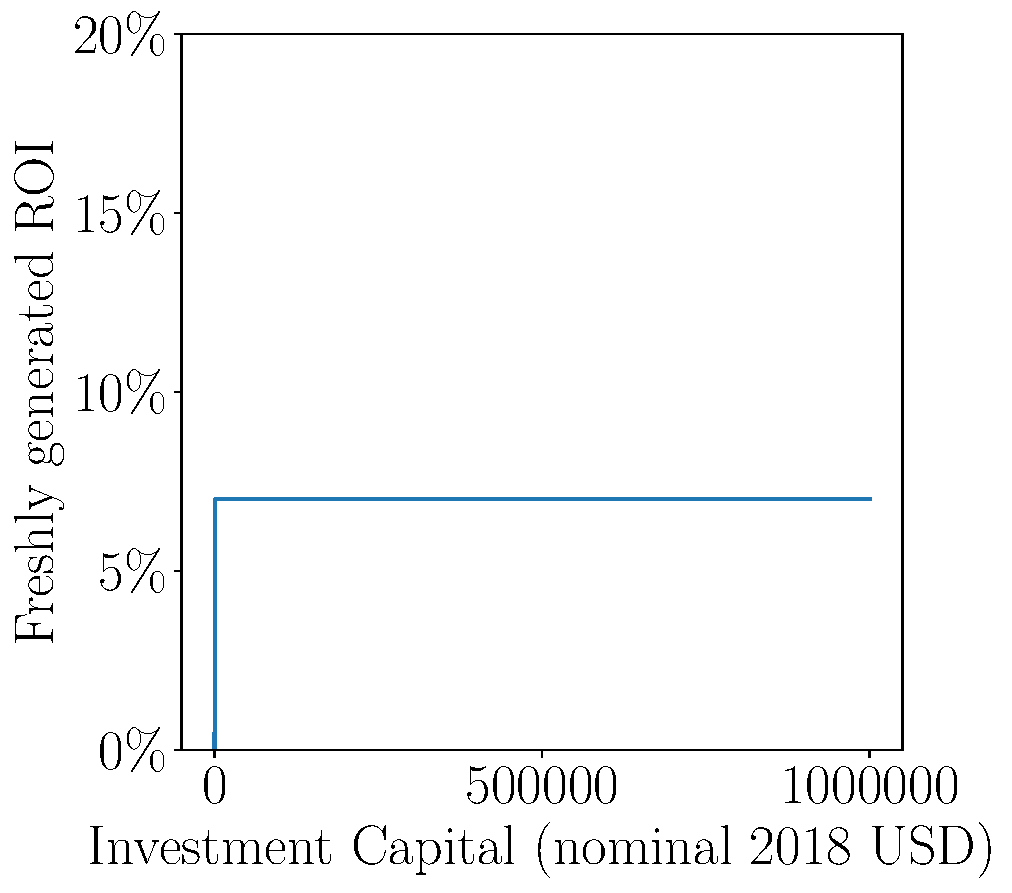
\includegraphics[width=0.4 \columnwidth,keepaspectratio]{figures/ideal.pdf}
%     \caption{The ideal egalitarian curve of an ideal cryptocurrency.}
%     \label{fig:ideal}
% \end{figure}

As an interesting thought experiment, consider the egalitarian curve which is
decreasing. In this case, the poor would receive proportionally more newly
created cryptocurrencies for every dollar they invest, \ie it would be a
perfectly fair redistribution of wealth from the rich to the poor. However, one
can quickly see that, in decentralized cryptocurrencies where the identities of
the participants are unknown, it is impossible to
hope for something better than the constant curve. Indeed, the fact that
decentralized cryptocurrencies allow anonymous generation of new
identities~\cite{douceur2002sybil}
allows a rich investor to split their investment into smaller ones.  Thus, if
the curve were ever to have a negative slope, the sum of the smaller splits of
the rich investment would achieve a higher gain. By the definition of the
curve, which mandates that it depicts the ROI of an \emph{optimal} investment,
this would be a contradiction. We following theorem makes the above intuition
more precise:

\begin{theorem}[Sybil strategies]\label{thm:sybil}
    Fix a cryptocurrency $c$ and an investment interval $d$. Given capital $v$,
    for every natural number $i \in \mathbb{N}^\star$, it
    holds that $f_{c,d}(v) \leq f_{c,d}(i \cdot v)$.
\end{theorem}

\begin{proof}
    We prove the statement via contradiction. Assume that for capital $v$
    exists a natural number $i \in \mathbb{N}^\star$ such that
    $f_{c,d}(v) > f_{c,d}(i \cdot v)$. Also assume that for
    capital $v$ the optimal strategy is $B'$, so: $\underset{B \in
    \mathbb{B}}{\max}{\mathbb{E}[B(v)]} = \mathbb{E}[B'(v)]$. Then, for capital
    $i \cdot v$ exists a strategy $B''$, such that the capital is split into $i$
    equally-sized parts and the strategy $B'$ is applied on each part. Given
    that the executions of the substrategies on these parts are independent,
    then the expected returns for the strategy $B''$ are:
    \begin{align}\label{eq:break-strategy}
        \mathbb{E}[B''(i \cdot v)] = i \cdot \mathbb{E}[B'(v)]  = i \cdot \underset{B \in \mathbb{B}}{\max}{\mathbb{E}[B(v)]}
    \end{align}
    It also holds that $B''$ is at best the optimal strategy, so:
    \begin{align}\label{eq:multi-strategy}
        \underset{B \in \mathbb{B}}{\max}{\mathbb{E}[B(i \cdot v)]} \geq \mathbb{E}[B''(i \cdot v)] \xRightarrow{\text{(\ref{eq:break-strategy})}}
        \underset{B \in \mathbb{B}}{\max}{\mathbb{E}[B(i \cdot v)]} \geq i \cdot \underset{B \in \mathbb{B}}{\max}{\mathbb{E}[B(v)]}
    \end{align}
    However, it should hold that:
    \begin{alignat}{2}
        f_{c,d}(v) &> f_{c,d}(i \cdot v) \Rightarrow \notag\\
        \frac{\underset{B \in \mathbb{B}}{\max}{\mathbb{E}[B(v)]} - v}{v} &> \frac{\underset{B \in \mathbb{B}}{\max}{\mathbb{E}[B(i \cdot v)]} - i \cdot v}{i \cdot v} \xRightarrow{\text{(\ref{eq:multi-strategy})}} \notag\\
        \frac{\underset{B \in \mathbb{B}}{\max}{\mathbb{E}[B(v)]} - v}{v} &> \frac{i \cdot \underset{B \in \mathbb{B}}{\max}{\mathbb{E}[B(v)]} - i \cdot v}{i \cdot v} \Rightarrow \notag\\
        \frac{\underset{B \in \mathbb{B}}{\max}{\mathbb{E}[B(v)]} - v}{v} &> \frac{\underset{B \in \mathbb{B}}{\max}{\mathbb{E}[B(v)]} - v}{v}
    \end{alignat}
    which is impossible.
\end{proof}

Using our definition of the egalitarian curve, we now define egalitarianism as
a concrete number. We begin by considering the initial capital $v$ as a random
variable following a certain distribution $\mathcal{D}$. Egalitarianism is
defined as the variance of the expected ROI when the capital is chosen from the
given distribution.

\begin{definition}[Egalitarianism]
  Given a cryptocurrency $c$, an investment period duration $d$ and an initial
  capital distribution $\mathcal{D}$, we define the \emph{egalitarianism} $e$ of $c$
  for investment duration $d$ under initial capital distribution $\mathcal{D}$
  as follows:

  \[
    e_{c,d,\mathcal{D}} = -\textsf{Var}_{v \gets \mathcal{D}}[f_{c,d}(v)]
  \]

  where $f$ is the egalitarian curve of $c$ for investment interval $d$ and the support of
  $\mathcal{D}$ is $[v_0, v_1]$.
\end{definition}

The intuition behind this definition is that, to have egalitarianism, the ROI
must remain the same across different capital investments. As such, any
deviation from the mean is non-egalitarian. Our notion allows the comparison of
the egalitarianism of different cryptocurrencies. Naturally, if the
egalitarianism of a certain cryptocurrency is \emph{higher} than another's, we
say that the former is \emph{more egalitarian} than the latter. Of course, to be
accurate, such comparisons must only be made after fixing the parameters $c$
and $d$ as well as the initial capital distribution $\mathcal{D}$.

Clearly a cryptocurrency with an ideal egalitarian curve is perfectly
egalitarian, as we now define.

\begin{definition}[Perfect egalitarianism]
  A cryptocurrency $c$ is \emph{perfectly egalitarian} for investment duration
  $d$ and initial capital distribution $\mathcal{D}$ if
  $e_{c,d,\mathcal{D}} = 0$.
\end{definition}
